% Created by tikzDevice version 0.12.6 on 2025-05-07 07:42:34
% !TEX encoding = UTF-8 Unicode
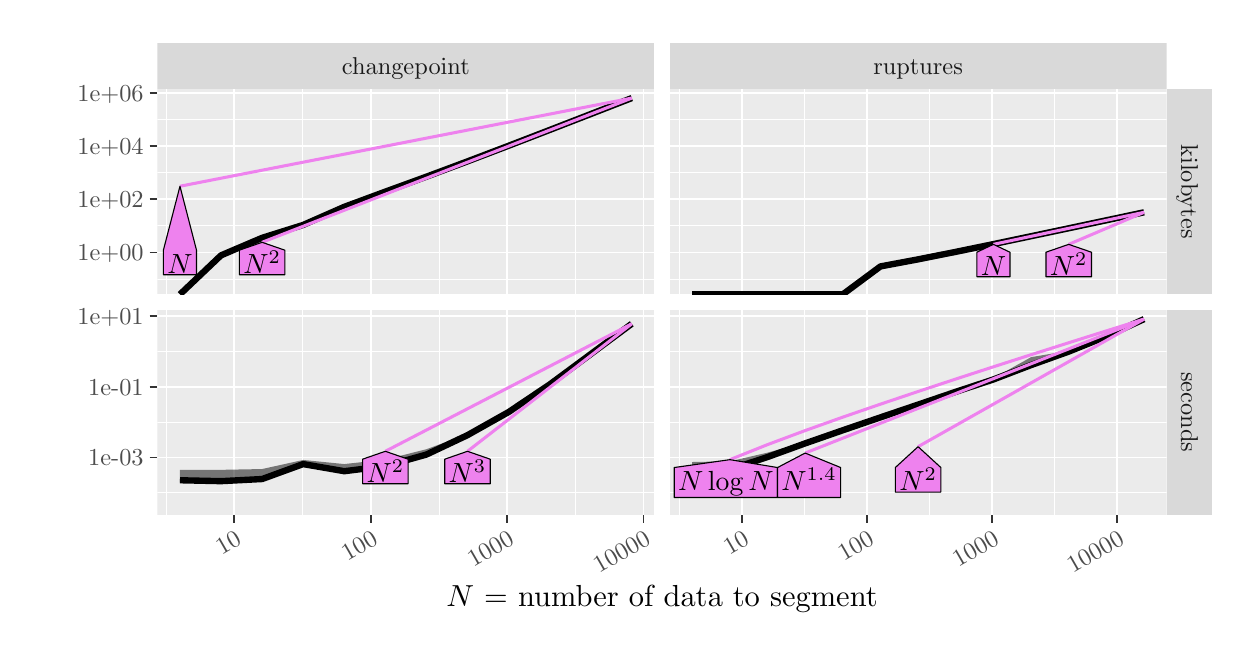
\begin{tikzpicture}[x=1pt,y=1pt]
\definecolor{fillColor}{RGB}{255,255,255}
\path[use as bounding box,fill=fillColor,fill opacity=0.00] (0,0) rectangle (433.62,216.81);
\begin{scope}
\path[clip] (  0.00,  0.00) rectangle (433.62,216.81);
\definecolor{drawColor}{RGB}{255,255,255}
\definecolor{fillColor}{RGB}{255,255,255}

\path[draw=drawColor,line width= 0.6pt,line join=round,line cap=round,fill=fillColor] ( -0.00,  0.00) rectangle (433.62,216.81);
\end{scope}
\begin{scope}
\path[clip] ( 46.86,120.44) rectangle (226.46,194.74);
\definecolor{fillColor}{gray}{0.92}

\path[fill=fillColor] ( 46.86,120.44) rectangle (226.46,194.74);
\definecolor{drawColor}{RGB}{255,255,255}

\path[draw=drawColor,line width= 0.3pt,line join=round] ( 46.86,125.99) --
	(226.46,125.99);

\path[draw=drawColor,line width= 0.3pt,line join=round] ( 46.86,145.23) --
	(226.46,145.23);

\path[draw=drawColor,line width= 0.3pt,line join=round] ( 46.86,164.47) --
	(226.46,164.47);

\path[draw=drawColor,line width= 0.3pt,line join=round] ( 46.86,183.70) --
	(226.46,183.70);

\path[draw=drawColor,line width= 0.3pt,line join=round] ( 50.00,120.44) --
	( 50.00,194.74);

\path[draw=drawColor,line width= 0.3pt,line join=round] ( 99.30,120.44) --
	( 99.30,194.74);

\path[draw=drawColor,line width= 0.3pt,line join=round] (148.61,120.44) --
	(148.61,194.74);

\path[draw=drawColor,line width= 0.3pt,line join=round] (197.91,120.44) --
	(197.91,194.74);

\path[draw=drawColor,line width= 0.6pt,line join=round] ( 46.86,135.61) --
	(226.46,135.61);

\path[draw=drawColor,line width= 0.6pt,line join=round] ( 46.86,154.85) --
	(226.46,154.85);

\path[draw=drawColor,line width= 0.6pt,line join=round] ( 46.86,174.08) --
	(226.46,174.08);

\path[draw=drawColor,line width= 0.6pt,line join=round] ( 46.86,193.32) --
	(226.46,193.32);

\path[draw=drawColor,line width= 0.6pt,line join=round] ( 74.65,120.44) --
	( 74.65,194.74);

\path[draw=drawColor,line width= 0.6pt,line join=round] (123.95,120.44) --
	(123.95,194.74);

\path[draw=drawColor,line width= 0.6pt,line join=round] (173.26,120.44) --
	(173.26,194.74);

\path[draw=drawColor,line width= 0.6pt,line join=round] (222.56,120.44) --
	(222.56,194.74);
\definecolor{drawColor}{RGB}{0,0,0}

\path[draw=drawColor,line width= 2.3pt,line join=round] ( 55.03,120.44) --
	( 69.87,134.54) --
	( 84.71,140.87) --
	( 99.55,145.53) --
	(114.40,152.07) --
	(129.24,157.56) --
	(144.08,162.96) --
	(158.92,168.49) --
	(173.77,174.13) --
	(188.61,179.84) --
	(203.45,185.59) --
	(218.29,191.36);
\definecolor{drawColor}{RGB}{238,130,238}

\path[draw=drawColor,line width= 1.1pt,line join=round] ( 84.71,139.25) --
	( 99.55,145.04) --
	(114.40,150.83) --
	(129.24,156.62) --
	(144.08,162.41) --
	(158.92,168.20) --
	(173.77,173.99) --
	(188.61,179.78) --
	(203.45,185.57) --
	(218.29,191.36);

\path[draw=drawColor,line width= 1.1pt,line join=round] ( 55.03,159.51) --
	( 69.87,162.41) --
	( 84.71,165.30) --
	( 99.55,168.20) --
	(114.40,171.09) --
	(129.24,173.99) --
	(144.08,176.89) --
	(158.92,179.78) --
	(173.77,182.68) --
	(188.61,185.57) --
	(203.45,188.47) --
	(218.29,191.36);
\end{scope}
\begin{scope}
\path[clip] ( 46.86,120.44) rectangle (226.46,194.74);
\definecolor{drawColor}{RGB}{0,0,0}
\definecolor{fillColor}{RGB}{238,130,238}

\path[draw=drawColor,line width= 0.4pt,line join=round,line cap=round,fill=fillColor] ( 76.48,136.40) --
	( 84.71,139.25) --
	( 92.94,136.40) --
	( 92.94,127.54) --
	( 76.48,127.54) --
	cycle;

\path[draw=drawColor,line width= 0.4pt,line join=round,line cap=round,fill=fillColor] ( 49.04,136.40) --
	( 55.03,159.51) --
	( 61.01,136.40) --
	( 61.01,127.54) --
	( 49.04,127.54) --
	cycle;

\node[text=drawColor,anchor=base,inner sep=0pt, outer sep=0pt, scale=  1.00] at ( 84.71,128.09) {$N^2$};

\node[text=drawColor,anchor=base,inner sep=0pt, outer sep=0pt, scale=  1.00] at ( 55.03,128.09) {$N$};
\end{scope}
\begin{scope}
\path[clip] ( 46.86, 40.64) rectangle (226.46,114.94);
\definecolor{fillColor}{gray}{0.92}

\path[fill=fillColor] ( 46.86, 40.64) rectangle (226.46,114.94);
\definecolor{drawColor}{RGB}{255,255,255}

\path[draw=drawColor,line width= 0.3pt,line join=round] ( 46.86, 48.79) --
	(226.46, 48.79);

\path[draw=drawColor,line width= 0.3pt,line join=round] ( 46.86, 74.31) --
	(226.46, 74.31);

\path[draw=drawColor,line width= 0.3pt,line join=round] ( 46.86, 99.82) --
	(226.46, 99.82);

\path[draw=drawColor,line width= 0.3pt,line join=round] ( 50.00, 40.64) --
	( 50.00,114.94);

\path[draw=drawColor,line width= 0.3pt,line join=round] ( 99.30, 40.64) --
	( 99.30,114.94);

\path[draw=drawColor,line width= 0.3pt,line join=round] (148.61, 40.64) --
	(148.61,114.94);

\path[draw=drawColor,line width= 0.3pt,line join=round] (197.91, 40.64) --
	(197.91,114.94);

\path[draw=drawColor,line width= 0.6pt,line join=round] ( 46.86, 61.55) --
	(226.46, 61.55);

\path[draw=drawColor,line width= 0.6pt,line join=round] ( 46.86, 87.07) --
	(226.46, 87.07);

\path[draw=drawColor,line width= 0.6pt,line join=round] ( 46.86,112.58) --
	(226.46,112.58);

\path[draw=drawColor,line width= 0.6pt,line join=round] ( 74.65, 40.64) --
	( 74.65,114.94);

\path[draw=drawColor,line width= 0.6pt,line join=round] (123.95, 40.64) --
	(123.95,114.94);

\path[draw=drawColor,line width= 0.6pt,line join=round] (173.26, 40.64) --
	(173.26,114.94);

\path[draw=drawColor,line width= 0.6pt,line join=round] (222.56, 40.64) --
	(222.56,114.94);
\definecolor{fillColor}{RGB}{0,0,0}

\path[fill=fillColor,fill opacity=0.50] ( 55.03, 56.99) --
	( 69.87, 57.03) --
	( 84.71, 57.32) --
	( 99.55, 60.60) --
	(114.40, 59.12) --
	(129.24, 60.73) --
	(144.08, 64.48) --
	(158.92, 69.92) --
	(173.77, 78.10) --
	(188.61, 89.04) --
	(203.45, 99.45) --
	(218.29,110.08) --
	(218.29,109.75) --
	(203.45, 98.66) --
	(188.61, 87.82) --
	(173.77, 77.86) --
	(158.92, 69.30) --
	(144.08, 62.34) --
	(129.24, 57.82) --
	(114.40, 55.88) --
	( 99.55, 58.18) --
	( 84.71, 53.31) --
	( 69.87, 52.48) --
	( 55.03, 52.46) --
	cycle;

\path[] ( 55.03, 56.99) --
	( 69.87, 57.03) --
	( 84.71, 57.32) --
	( 99.55, 60.60) --
	(114.40, 59.12) --
	(129.24, 60.73) --
	(144.08, 64.48) --
	(158.92, 69.92) --
	(173.77, 78.10) --
	(188.61, 89.04) --
	(203.45, 99.45) --
	(218.29,110.08);

\path[] (218.29,109.75) --
	(203.45, 98.66) --
	(188.61, 87.82) --
	(173.77, 77.86) --
	(158.92, 69.30) --
	(144.08, 62.34) --
	(129.24, 57.82) --
	(114.40, 55.88) --
	( 99.55, 58.18) --
	( 84.71, 53.31) --
	( 69.87, 52.48) --
	( 55.03, 52.46);
\definecolor{drawColor}{RGB}{0,0,0}

\path[draw=drawColor,line width= 2.3pt,line join=round] ( 55.03, 53.27) --
	( 69.87, 52.94) --
	( 84.71, 53.71) --
	( 99.55, 59.11) --
	(114.40, 56.54) --
	(129.24, 58.38) --
	(144.08, 62.55) --
	(158.92, 69.56) --
	(173.77, 77.91) --
	(188.61, 87.87) --
	(203.45, 98.84) --
	(218.29,109.81);
\definecolor{drawColor}{RGB}{238,130,238}

\path[draw=drawColor,line width= 1.1pt,line join=round] (129.24, 63.73) --
	(144.08, 71.41) --
	(158.92, 79.09) --
	(173.77, 86.77) --
	(188.61, 94.45) --
	(203.45,102.13) --
	(218.29,109.81);

\path[draw=drawColor,line width= 1.1pt,line join=round] (158.92, 63.73) --
	(173.77, 75.25) --
	(188.61, 86.77) --
	(203.45, 98.29) --
	(218.29,109.81);
\end{scope}
\begin{scope}
\path[clip] ( 46.86, 40.64) rectangle (226.46,114.94);
\definecolor{drawColor}{RGB}{0,0,0}
\definecolor{fillColor}{RGB}{238,130,238}

\path[draw=drawColor,line width= 0.4pt,line join=round,line cap=round,fill=fillColor] (121.01, 60.88) --
	(129.24, 63.73) --
	(137.47, 60.88) --
	(137.47, 52.02) --
	(121.01, 52.02) --
	cycle;

\path[draw=drawColor,line width= 0.4pt,line join=round,line cap=round,fill=fillColor] (150.70, 60.88) --
	(158.92, 63.73) --
	(167.15, 60.88) --
	(167.15, 52.02) --
	(150.70, 52.02) --
	cycle;

\node[text=drawColor,anchor=base,inner sep=0pt, outer sep=0pt, scale=  1.00] at (129.24, 52.57) {$N^2$};

\node[text=drawColor,anchor=base,inner sep=0pt, outer sep=0pt, scale=  1.00] at (158.92, 52.57) {$N^3$};
\end{scope}
\begin{scope}
\path[clip] (231.96,120.44) rectangle (411.55,194.74);
\definecolor{fillColor}{gray}{0.92}

\path[fill=fillColor] (231.96,120.44) rectangle (411.55,194.74);
\definecolor{drawColor}{RGB}{255,255,255}

\path[draw=drawColor,line width= 0.3pt,line join=round] (231.96,125.99) --
	(411.55,125.99);

\path[draw=drawColor,line width= 0.3pt,line join=round] (231.96,145.23) --
	(411.55,145.23);

\path[draw=drawColor,line width= 0.3pt,line join=round] (231.96,164.47) --
	(411.55,164.47);

\path[draw=drawColor,line width= 0.3pt,line join=round] (231.96,183.70) --
	(411.55,183.70);

\path[draw=drawColor,line width= 0.3pt,line join=round] (235.51,120.44) --
	(235.51,194.74);

\path[draw=drawColor,line width= 0.3pt,line join=round] (280.70,120.44) --
	(280.70,194.74);

\path[draw=drawColor,line width= 0.3pt,line join=round] (325.90,120.44) --
	(325.90,194.74);

\path[draw=drawColor,line width= 0.3pt,line join=round] (371.10,120.44) --
	(371.10,194.74);

\path[draw=drawColor,line width= 0.6pt,line join=round] (231.96,135.61) --
	(411.55,135.61);

\path[draw=drawColor,line width= 0.6pt,line join=round] (231.96,154.85) --
	(411.55,154.85);

\path[draw=drawColor,line width= 0.6pt,line join=round] (231.96,174.08) --
	(411.55,174.08);

\path[draw=drawColor,line width= 0.6pt,line join=round] (231.96,193.32) --
	(411.55,193.32);

\path[draw=drawColor,line width= 0.6pt,line join=round] (258.11,120.44) --
	(258.11,194.74);

\path[draw=drawColor,line width= 0.6pt,line join=round] (303.30,120.44) --
	(303.30,194.74);

\path[draw=drawColor,line width= 0.6pt,line join=round] (348.50,120.44) --
	(348.50,194.74);

\path[draw=drawColor,line width= 0.6pt,line join=round] (393.69,120.44) --
	(393.69,194.74);
\definecolor{drawColor}{RGB}{0,0,0}

\path[draw=drawColor,line width= 2.3pt,line join=round] (240.12,120.44) --
	(253.73,120.44) --
	(267.33,120.44) --
	(280.94,120.44) --
	(294.54,120.44) --
	(308.15,130.54) --
	(321.75,133.09) --
	(335.36,135.80) --
	(348.96,138.60) --
	(362.57,141.45) --
	(376.17,144.32) --
	(389.78,147.21) --
	(403.39,150.09);
\definecolor{drawColor}{RGB}{238,130,238}

\path[draw=drawColor,line width= 1.1pt,line join=round] (376.17,138.51) --
	(389.78,144.30) --
	(403.39,150.09);

\path[draw=drawColor,line width= 1.1pt,line join=round] (348.96,138.51) --
	(362.57,141.41) --
	(376.17,144.30) --
	(389.78,147.20) --
	(403.39,150.09);
\end{scope}
\begin{scope}
\path[clip] (231.96,120.44) rectangle (411.55,194.74);
\definecolor{drawColor}{RGB}{0,0,0}
\definecolor{fillColor}{RGB}{238,130,238}

\path[draw=drawColor,line width= 0.4pt,line join=round,line cap=round,fill=fillColor] (367.95,135.67) --
	(376.17,138.51) --
	(384.40,135.67) --
	(384.40,126.80) --
	(367.95,126.80) --
	cycle;

\path[draw=drawColor,line width= 0.4pt,line join=round,line cap=round,fill=fillColor] (342.98,135.67) --
	(348.96,138.51) --
	(354.95,135.67) --
	(354.95,126.80) --
	(342.98,126.80) --
	cycle;

\node[text=drawColor,anchor=base,inner sep=0pt, outer sep=0pt, scale=  1.00] at (376.17,127.36) {$N^2$};

\node[text=drawColor,anchor=base,inner sep=0pt, outer sep=0pt, scale=  1.00] at (348.96,127.36) {$N$};
\end{scope}
\begin{scope}
\path[clip] (231.96, 40.64) rectangle (411.55,114.94);
\definecolor{fillColor}{gray}{0.92}

\path[fill=fillColor] (231.96, 40.64) rectangle (411.55,114.94);
\definecolor{drawColor}{RGB}{255,255,255}

\path[draw=drawColor,line width= 0.3pt,line join=round] (231.96, 48.79) --
	(411.55, 48.79);

\path[draw=drawColor,line width= 0.3pt,line join=round] (231.96, 74.31) --
	(411.55, 74.31);

\path[draw=drawColor,line width= 0.3pt,line join=round] (231.96, 99.82) --
	(411.55, 99.82);

\path[draw=drawColor,line width= 0.3pt,line join=round] (235.51, 40.64) --
	(235.51,114.94);

\path[draw=drawColor,line width= 0.3pt,line join=round] (280.70, 40.64) --
	(280.70,114.94);

\path[draw=drawColor,line width= 0.3pt,line join=round] (325.90, 40.64) --
	(325.90,114.94);

\path[draw=drawColor,line width= 0.3pt,line join=round] (371.10, 40.64) --
	(371.10,114.94);

\path[draw=drawColor,line width= 0.6pt,line join=round] (231.96, 61.55) --
	(411.55, 61.55);

\path[draw=drawColor,line width= 0.6pt,line join=round] (231.96, 87.07) --
	(411.55, 87.07);

\path[draw=drawColor,line width= 0.6pt,line join=round] (231.96,112.58) --
	(411.55,112.58);

\path[draw=drawColor,line width= 0.6pt,line join=round] (258.11, 40.64) --
	(258.11,114.94);

\path[draw=drawColor,line width= 0.6pt,line join=round] (303.30, 40.64) --
	(303.30,114.94);

\path[draw=drawColor,line width= 0.6pt,line join=round] (348.50, 40.64) --
	(348.50,114.94);

\path[draw=drawColor,line width= 0.6pt,line join=round] (393.69, 40.64) --
	(393.69,114.94);
\definecolor{fillColor}{RGB}{0,0,0}

\path[fill=fillColor,fill opacity=0.50] (240.12, 59.86) --
	(253.73, 60.11) --
	(267.33, 63.24) --
	(280.94, 67.07) --
	(294.54, 71.40) --
	(308.15, 76.33) --
	(321.75, 81.19) --
	(335.36, 85.66) --
	(348.96, 90.13) --
	(362.57, 97.75) --
	(376.17,100.03) --
	(389.78,105.46) --
	(403.39,111.56) --
	(403.39,111.44) --
	(389.78,105.19) --
	(376.17, 99.67) --
	(362.57, 94.81) --
	(348.96, 89.66) --
	(335.36, 84.90) --
	(321.75, 80.54) --
	(308.15, 75.94) --
	(294.54, 71.18) --
	(280.94, 66.41) --
	(267.33, 61.49) --
	(253.73, 57.03) --
	(240.12, 53.14) --
	cycle;

\path[] (240.12, 59.86) --
	(253.73, 60.11) --
	(267.33, 63.24) --
	(280.94, 67.07) --
	(294.54, 71.40) --
	(308.15, 76.33) --
	(321.75, 81.19) --
	(335.36, 85.66) --
	(348.96, 90.13) --
	(362.57, 97.75) --
	(376.17,100.03) --
	(389.78,105.46) --
	(403.39,111.56);

\path[] (403.39,111.44) --
	(389.78,105.19) --
	(376.17, 99.67) --
	(362.57, 94.81) --
	(348.96, 89.66) --
	(335.36, 84.90) --
	(321.75, 80.54) --
	(308.15, 75.94) --
	(294.54, 71.18) --
	(280.94, 66.41) --
	(267.33, 61.49) --
	(253.73, 57.03) --
	(240.12, 53.14);
\definecolor{drawColor}{RGB}{0,0,0}

\path[draw=drawColor,line width= 2.3pt,line join=round] (240.12, 53.54) --
	(253.73, 57.15) --
	(267.33, 61.65) --
	(280.94, 66.59) --
	(294.54, 71.33) --
	(308.15, 75.99) --
	(321.75, 80.60) --
	(335.36, 85.23) --
	(348.96, 89.69) --
	(362.57, 94.88) --
	(376.17, 99.75) --
	(389.78,105.24) --
	(403.39,111.49);
\definecolor{drawColor}{RGB}{238,130,238}

\path[draw=drawColor,line width= 1.1pt,line join=round] (253.73, 60.71) --
	(267.33, 66.14) --
	(280.94, 71.22) --
	(294.54, 76.07) --
	(308.15, 80.76) --
	(321.75, 85.34) --
	(335.36, 89.84) --
	(348.96, 94.26) --
	(362.57, 98.63) --
	(376.17,102.95) --
	(389.78,107.24) --
	(403.39,111.49);

\path[draw=drawColor,line width= 1.1pt,line join=round] (280.94, 63.10) --
	(294.54, 68.47) --
	(308.15, 73.85) --
	(321.75, 79.23) --
	(335.36, 84.60) --
	(348.96, 89.98) --
	(362.57, 95.36) --
	(376.17,100.73) --
	(389.78,106.11) --
	(403.39,111.49);

\path[draw=drawColor,line width= 1.1pt,line join=round] (321.75, 65.40) --
	(335.36, 73.08) --
	(348.96, 80.76) --
	(362.57, 88.44) --
	(376.17, 96.12) --
	(389.78,103.81) --
	(403.39,111.49);
\end{scope}
\begin{scope}
\path[clip] (231.96, 40.64) rectangle (411.55,114.94);
\definecolor{drawColor}{RGB}{0,0,0}
\definecolor{fillColor}{RGB}{238,130,238}

\path[draw=drawColor,line width= 0.4pt,line join=round,line cap=round,fill=fillColor] (233.62, 57.86) --
	(253.73, 60.71) --
	(270.96, 57.86) --
	(270.96, 47.05) --
	(233.62, 47.05) --
	cycle;

\path[draw=drawColor,line width= 0.4pt,line join=round,line cap=round,fill=fillColor] (270.96, 57.86) --
	(280.94, 63.10) --
	(293.78, 57.86) --
	(293.78, 47.05) --
	(270.96, 47.05) --
	cycle;

\path[draw=drawColor,line width= 0.4pt,line join=round,line cap=round,fill=fillColor] (313.52, 57.86) --
	(321.75, 65.40) --
	(329.98, 57.86) --
	(329.98, 49.00) --
	(313.52, 49.00) --
	cycle;

\node[text=drawColor,anchor=base,inner sep=0pt, outer sep=0pt, scale=  1.00] at (252.29, 49.55) {$N \log N$};

\node[text=drawColor,anchor=base,inner sep=0pt, outer sep=0pt, scale=  1.00] at (282.37, 49.55) {$N^{1.4}$};

\node[text=drawColor,anchor=base,inner sep=0pt, outer sep=0pt, scale=  1.00] at (321.75, 49.55) {$N^2$};
\end{scope}
\begin{scope}
\path[clip] ( 46.86,194.74) rectangle (226.46,211.31);
\definecolor{fillColor}{gray}{0.85}

\path[fill=fillColor] ( 46.86,194.74) rectangle (226.46,211.31);
\definecolor{drawColor}{gray}{0.10}

\node[text=drawColor,anchor=base,inner sep=0pt, outer sep=0pt, scale=  0.88] at (136.66,199.99) {changepoint};
\end{scope}
\begin{scope}
\path[clip] (231.96,194.74) rectangle (411.55,211.31);
\definecolor{fillColor}{gray}{0.85}

\path[fill=fillColor] (231.96,194.74) rectangle (411.55,211.31);
\definecolor{drawColor}{gray}{0.10}

\node[text=drawColor,anchor=base,inner sep=0pt, outer sep=0pt, scale=  0.88] at (321.75,199.99) {ruptures};
\end{scope}
\begin{scope}
\path[clip] (411.55,120.44) rectangle (428.12,194.74);
\definecolor{fillColor}{gray}{0.85}

\path[fill=fillColor] (411.55,120.44) rectangle (428.12,194.74);
\definecolor{drawColor}{gray}{0.10}

\node[text=drawColor,rotate=-90.00,anchor=base,inner sep=0pt, outer sep=0pt, scale=  0.88] at (416.80,157.59) {kilobytes};
\end{scope}
\begin{scope}
\path[clip] (411.55, 40.64) rectangle (428.12,114.94);
\definecolor{fillColor}{gray}{0.85}

\path[fill=fillColor] (411.55, 40.64) rectangle (428.12,114.94);
\definecolor{drawColor}{gray}{0.10}

\node[text=drawColor,rotate=-90.00,anchor=base,inner sep=0pt, outer sep=0pt, scale=  0.88] at (416.80, 77.79) {seconds};
\end{scope}
\begin{scope}
\path[clip] (  0.00,  0.00) rectangle (433.62,216.81);
\definecolor{drawColor}{gray}{0.20}

\path[draw=drawColor,line width= 0.6pt,line join=round] ( 74.65, 37.89) --
	( 74.65, 40.64);

\path[draw=drawColor,line width= 0.6pt,line join=round] (123.95, 37.89) --
	(123.95, 40.64);

\path[draw=drawColor,line width= 0.6pt,line join=round] (173.26, 37.89) --
	(173.26, 40.64);

\path[draw=drawColor,line width= 0.6pt,line join=round] (222.56, 37.89) --
	(222.56, 40.64);
\end{scope}
\begin{scope}
\path[clip] (  0.00,  0.00) rectangle (433.62,216.81);
\definecolor{drawColor}{gray}{0.30}

\node[text=drawColor,rotate= 30.00,anchor=base east,inner sep=0pt, outer sep=0pt, scale=  0.88] at ( 77.68, 30.44) {10};

\node[text=drawColor,rotate= 30.00,anchor=base east,inner sep=0pt, outer sep=0pt, scale=  0.88] at (126.98, 30.44) {100};

\node[text=drawColor,rotate= 30.00,anchor=base east,inner sep=0pt, outer sep=0pt, scale=  0.88] at (176.29, 30.44) {1000};

\node[text=drawColor,rotate= 30.00,anchor=base east,inner sep=0pt, outer sep=0pt, scale=  0.88] at (225.59, 30.44) {10000};
\end{scope}
\begin{scope}
\path[clip] (  0.00,  0.00) rectangle (433.62,216.81);
\definecolor{drawColor}{gray}{0.20}

\path[draw=drawColor,line width= 0.6pt,line join=round] (258.11, 37.89) --
	(258.11, 40.64);

\path[draw=drawColor,line width= 0.6pt,line join=round] (303.30, 37.89) --
	(303.30, 40.64);

\path[draw=drawColor,line width= 0.6pt,line join=round] (348.50, 37.89) --
	(348.50, 40.64);

\path[draw=drawColor,line width= 0.6pt,line join=round] (393.69, 37.89) --
	(393.69, 40.64);
\end{scope}
\begin{scope}
\path[clip] (  0.00,  0.00) rectangle (433.62,216.81);
\definecolor{drawColor}{gray}{0.30}

\node[text=drawColor,rotate= 30.00,anchor=base east,inner sep=0pt, outer sep=0pt, scale=  0.88] at (261.14, 30.44) {10};

\node[text=drawColor,rotate= 30.00,anchor=base east,inner sep=0pt, outer sep=0pt, scale=  0.88] at (306.33, 30.44) {100};

\node[text=drawColor,rotate= 30.00,anchor=base east,inner sep=0pt, outer sep=0pt, scale=  0.88] at (351.53, 30.44) {1000};

\node[text=drawColor,rotate= 30.00,anchor=base east,inner sep=0pt, outer sep=0pt, scale=  0.88] at (396.72, 30.44) {10000};
\end{scope}
\begin{scope}
\path[clip] (  0.00,  0.00) rectangle (433.62,216.81);
\definecolor{drawColor}{gray}{0.30}

\node[text=drawColor,anchor=base east,inner sep=0pt, outer sep=0pt, scale=  0.88] at ( 41.91,132.58) {1e+00};

\node[text=drawColor,anchor=base east,inner sep=0pt, outer sep=0pt, scale=  0.88] at ( 41.91,151.82) {1e+02};

\node[text=drawColor,anchor=base east,inner sep=0pt, outer sep=0pt, scale=  0.88] at ( 41.91,171.05) {1e+04};

\node[text=drawColor,anchor=base east,inner sep=0pt, outer sep=0pt, scale=  0.88] at ( 41.91,190.29) {1e+06};
\end{scope}
\begin{scope}
\path[clip] (  0.00,  0.00) rectangle (433.62,216.81);
\definecolor{drawColor}{gray}{0.20}

\path[draw=drawColor,line width= 0.6pt,line join=round] ( 44.11,135.61) --
	( 46.86,135.61);

\path[draw=drawColor,line width= 0.6pt,line join=round] ( 44.11,154.85) --
	( 46.86,154.85);

\path[draw=drawColor,line width= 0.6pt,line join=round] ( 44.11,174.08) --
	( 46.86,174.08);

\path[draw=drawColor,line width= 0.6pt,line join=round] ( 44.11,193.32) --
	( 46.86,193.32);
\end{scope}
\begin{scope}
\path[clip] (  0.00,  0.00) rectangle (433.62,216.81);
\definecolor{drawColor}{gray}{0.30}

\node[text=drawColor,anchor=base east,inner sep=0pt, outer sep=0pt, scale=  0.88] at ( 41.91, 58.52) {1e-03};

\node[text=drawColor,anchor=base east,inner sep=0pt, outer sep=0pt, scale=  0.88] at ( 41.91, 84.04) {1e-01};

\node[text=drawColor,anchor=base east,inner sep=0pt, outer sep=0pt, scale=  0.88] at ( 41.91,109.55) {1e+01};
\end{scope}
\begin{scope}
\path[clip] (  0.00,  0.00) rectangle (433.62,216.81);
\definecolor{drawColor}{gray}{0.20}

\path[draw=drawColor,line width= 0.6pt,line join=round] ( 44.11, 61.55) --
	( 46.86, 61.55);

\path[draw=drawColor,line width= 0.6pt,line join=round] ( 44.11, 87.07) --
	( 46.86, 87.07);

\path[draw=drawColor,line width= 0.6pt,line join=round] ( 44.11,112.58) --
	( 46.86,112.58);
\end{scope}
\begin{scope}
\path[clip] (  0.00,  0.00) rectangle (433.62,216.81);
\definecolor{drawColor}{RGB}{0,0,0}

\node[text=drawColor,anchor=base,inner sep=0pt, outer sep=0pt, scale=  1.10] at (229.21,  7.64) {$N$ = number of data to segment};
\end{scope}
\end{tikzpicture}
